\chapter{द्वि-घटकी द्रव--वाष्प आरेख और आसवन}\label{ch:b2:liquid-vapour-diagrams}

ताँबे का आसवन-पात्र कुछ प्रतिशत ऐल्कोहॉल वाली वाइन को कई गुना तेज़ स्पिरिट
में बदल देता है; रिफ़ाइनरी का स्तंभ कच्चे तेल को उसके अंशों में, गैस से
भारी ईंधन तक, बाँट देता है। दोनों एक ही तथ्य पर टिके हैं: उबलते मिश्रण के ऊपर की वाष्प
द्रव की तुलना में अधिक वाष्पशील घटक में समृद्ध होती है। वाष्पन और संघनन
पर्याप्त बार दोहराइए और पृथक्करण जितना चाहें उतना तीक्ष्ण हो जाता है --- एक
अपवाद के साथ: कोई भी आसवन, स्तंभ चाहे जितना लंबा हो, एथेनॉल को द्रव्यमान के अनुसार लगभग 95
प्रतिशत से आगे नहीं ले जाता। यह अध्याय वे आरेख खींचता है जो बताते हैं कि दो द्रवों का मिश्रण
कैसे उबलता है, और उनका उपयोग स्तंभ का अभिकल्पन करने और यह देखने में करता है कि उसे कहाँ रुकना पड़ता है।

\begin{recall}
\Cref{ch:b2:chemical-potential}: \omterm{def:b2:chemical-potential:chemical-potential}{रासायनिक विभव}, \omterm{thm:b2:chemical-potential:raoult}{राउल्ट का नियम} और
\omterm{def:b2:chemical-potential:ideal-mixture}{आदर्श मिश्रण}, \omterm{def:b2:chemical-potential:activity-coefficient}{सक्रियता गुणांक} और \omterm{thm:b2:chemical-potential:raoult}{राउल्ट के नियम} से विचलन,
गिब्स--ड्यूहेम संबंध। \Cref{ch:b2:equilibrium-shifts}: \omterm{def:b2:equilibrium-shifts:variance}{स्वातंत्र्य कोटि}।
प्रथम वर्ष का खंड, प्रयोगशाला तकनीकों पर: सरल आसवन, मिश्रणीय और
अमिश्रणीय द्रव। विद्यालय का खंड: आसवन और जल-आसवन।
\end{recall}

\begin{omfigure}
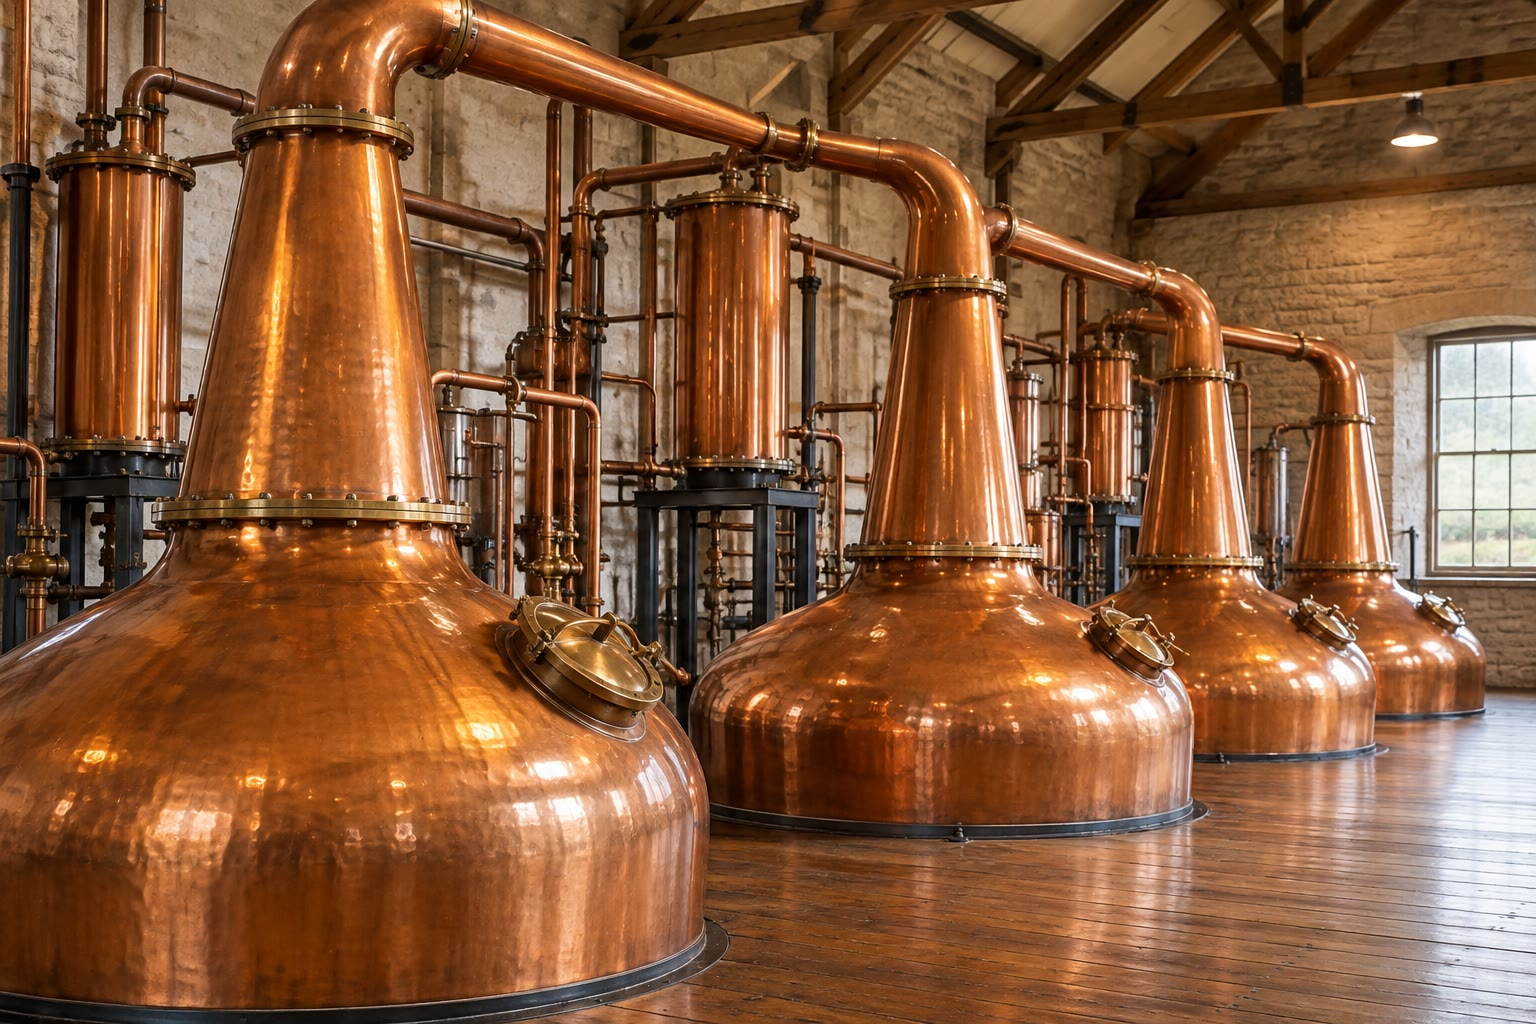
\includegraphics[width=0.62\linewidth]{images/book3/ai/b2-07-pot-stills.jpg}

{\small किसी आसवनी में ताँबे के आसवन-पात्र। किण्वित घोल का हर भार
उबाला जाता है और उसकी वाष्प संघनित की जाती है: पहला आसुत घोल की तुलना में
एथेनॉल में कई गुना समृद्ध होता है, और दूसरा आसवन उसे और सांद्र करता है।}
\end{omfigure}

\section{आदर्श मिश्रण}

इस अध्याय में दोनों द्रवों को 1 (अधिक वाष्पशील, निम्नतर
क्वथनांक वाला) और 2 क्रमांक दिए गए हैं; $x$ द्रव में 1 का मोल अंश है, $y$
वाष्प में उसका मोल अंश, जिसे आदर्श गैस माना जाता है।

\begin{definition}[द्वि-घटकी आरेख]\label{def:b2:liquid-vapour-diagrams:binary-diagram}
\emph{द्वि-घटकी आरेख}\index{द्वि-घटकी आरेख} दो घटकों के मिश्रण के लिए
दिखाता है कि कौन-सी प्रावस्थाएँ किन संघटनों के साथ उपस्थित हैं, समग्र संघटन
और एक अन्य चर के फलन के रूप में।
\emph{समदाबी आरेख}\index{समदाबी आरेख} नियत दाब पर तल
(संघटन, ताप) में खींचा जाता है; \emph{समतापी
आरेख}\index{समतापी आरेख} नियत ताप पर तल (संघटन, दाब) में।
\end{definition}

\begin{definition}[बुलबुला वक्र और ओस वक्र]\label{def:b2:liquid-vapour-diagrams:bubble-dew}
द्रव--वाष्प आरेख पर \emph{बुलबुला वक्र}\index{बुलबुला वक्र} वाष्प के साथ
साम्य में द्रव का संघटन देता है, \emph{ओस
वक्र}\index{ओस वक्र} द्रव के साथ साम्य में वाष्प का संघटन। नियत दाब पर दिए गए
संघटन वाले मिश्रण के लिए \emph{बुलबुला
बिंदु}\index{बुलबुला बिंदु} वह ताप है जिस पर गर्म करने पर वाष्प का पहला बुलबुला
प्रकट होता है, \emph{ओसांक}\index{ओसांक} वह
ताप जिस पर वाष्प को ठंडा करने पर द्रव की पहली बूँद प्रकट होती है।
\end{definition}

\begin{proposition}[आदर्श वक्र]\label{prop:b2:liquid-vapour-diagrams:ideal-curves}
ताप $T$ पर किसी \omterm{def:b2:chemical-potential:ideal-mixture}{आदर्श मिश्रण} के लिए, जहाँ $p_1^*$ और $p_2^*$ शुद्ध द्रवों के वाष्प
दाब हैं, \omterm{def:b2:liquid-vapour-diagrams:binary-diagram}{समतापी आरेख} का \omterm{def:b2:liquid-vapour-diagrams:bubble-dew}{बुलबुला वक्र}
सरल रेखा $p = p_2^* + x(p_1^* - p_2^*)$ है, और \omterm{def:b2:liquid-vapour-diagrams:bubble-dew}{ओस वक्र} यह
अतिपरवलय है:
\[
  p = \frac{1}{y/p_1^* + (1 - y)/p_2^*} .
\]
\end{proposition}

\begin{proof}
\omterm{thm:b2:chemical-potential:raoult}{राउल्ट का नियम} आंशिक दाब $p_1 = xp_1^*$ और $p_2 = (1 -
x)p_2^*$ देता है; उनका योग कुल दाब है, जो $x$ में रैखिक है। वाष्प में
$y = p_1/p$, अतः $x = yp/p_1^*$ और $1 - x = (1 - y)p/p_2^*$; जोड़ने पर
$1 = p\,[y/p_1^* + (1 - y)/p_2^*]$।
\end{proof}

\begin{proposition}[वाष्प अधिक वाष्पशील घटक में समृद्ध होती है]\label{prop:b2:liquid-vapour-diagrams:richer}
$p_1^* > p_2^*$ और $0 < x < 1$ वाले \omterm{def:b2:chemical-potential:ideal-mixture}{आदर्श मिश्रण} के लिए $y > x$।
\end{proposition}

\begin{proof}
$y = xp_1^*/p$, जहाँ $p = xp_1^* + (1 - x)p_2^* < p_1^*$, क्योंकि $p$,
$p_1^*$ और $p_2^*$ का भारित माध्य है, उनके ठीक बीच में। अतः $y >
x$।
\end{proof}

\omterm{def:b2:liquid-vapour-diagrams:binary-diagram}{समदाबी आरेख} वह है जो आसवन का वर्णन करता है, जो वायुमंडलीय दाब पर
चलता है। इसका कोई सरल सूत्र नहीं: दोनों क्वथनांकों के बीच के हर ताप के लिए
$p_1^*(T)$ और $p_2^*(T)$ परिकलित किए जाते हैं (यहाँ
एंटोइन समीकरण, $\log_{10}(p^*/\unit{bar}) = A - B/(T + C)$, से, जो
मापे गए वाष्प दाबों पर समंजित है), और फिर द्रव तथा वाष्प के वे संघटन जो
\qty{1.013}{bar} का कुल दाब देते हैं:
\[
  x = \frac{p - p_2^*(T)}{p_1^*(T) - p_2^*(T)}, \qquad y = \frac{x\,p_1^*(T)}{p} .
\]
\omterm{def:b2:liquid-vapour-diagrams:bubble-dew}{बुलबुला वक्र} अब सरल रेखा नहीं है; \omterm{def:b2:liquid-vapour-diagrams:bubble-dew}{ओस वक्र} अब भी उसके ऊपर है,
और वाष्प अब भी हल्के घटक में समृद्ध है।

\begin{example}[\qty{90}{\degreeCelsius} पर बेन्ज़ीन और टॉलूईन]\label{ex:b2:liquid-vapour-diagrams:benzene-toluene}
बेन्ज़ीन और टॉलूईन लगभग \omterm{def:b2:chemical-potential:ideal-mixture}{आदर्श मिश्रण} बनाते हैं। \qty{90}{\degreeCelsius} पर
एंटोइन समीकरण $p_1^* = \qty{1.361}{bar}$ (बेन्ज़ीन) और $p_2^* =
\qty{0.542}{bar}$ (टॉलूईन) देते हैं। \qty{1.013}{bar} पर: $x = (1.013 - 0.542)/(1.361 -
0.542) = 0.575$ और $y = 0.575 \times 1.361/1.013 = 0.773$। 57.5~\%
बेन्ज़ीन (मोल में) वाला द्रव \qty{90}{\degreeCelsius} पर उबलता है और
77~\% की वाष्प देता है।
% ledger: antoine:benzene.A, antoine:benzene.B, antoine:benzene.C, antoine:toluene.A, antoine:toluene.B, antoine:toluene.C
\end{example}

\begin{omfigure}
\begin{tikzpicture}
\begin{axis}[omphase, width=0.47\linewidth, height=6cm, ymin=78, ymax=113,
  xlabel={$x$, $y$ (बेन्ज़ीन)}, ylabel={$T$ (\unit{\degreeCelsius})},
  title={\small समदाबी, \qty{1.013}{bar}}]
\addplot[omliquidus] table[x=x, y=T] {figdata/out/bachelor-2-liquid-vapour-a.dat};
\addplot[omsolidus] table[x=y, y=T] {figdata/out/bachelor-2-liquid-vapour-a.dat};
\draw[tieline] (axis cs:0.405,95) -- (axis cs:0.626,95);
\fill (axis cs:0.5,95) circle (1.3pt);
\draw[->, thick] (axis cs:0.5,82) -- (axis cs:0.5,104) node[above, font=\scriptsize] {तापन};
\node[font=\scriptsize] at (axis cs:0.2,85) {द्रव};
\node[font=\scriptsize] at (axis cs:0.85,108) {वाष्प};
\node[font=\scriptsize, omDef, anchor=north] at (axis cs:0.22,96) {बुलबुला};
\node[font=\scriptsize, omThm, anchor=south west] at (axis cs:0.62,101) {ओस};
\end{axis}
\end{tikzpicture}\hfill
\begin{tikzpicture}
\begin{axis}[omphase, width=0.47\linewidth, height=6cm, ymin=0.3, ymax=1.1,
  xlabel={$x$, $y$ (बेन्ज़ीन)}, ylabel={$p$ (\unit{bar})},
  title={\small समतापी, \qty{80}{\degreeCelsius}}]
\addplot[omliquidus] table[x=x, y=pbub] {figdata/out/bachelor-2-liquid-vapour-b.dat};
\addplot[omsolidus] table[x=x, y=pdew] {figdata/out/bachelor-2-liquid-vapour-b.dat};
\node[font=\scriptsize] at (axis cs:0.75,0.98) {द्रव};
\node[font=\scriptsize] at (axis cs:0.2,0.36) {वाष्प};
\end{axis}
\end{tikzpicture}

{\small बेन्ज़ीन--टॉलूईन, \omterm{thm:b2:chemical-potential:raoult}{राउल्ट के नियम} और एंटोइन
समीकरणों से परिकलित। बाएँ, वायुमंडलीय दाब पर: \omterm{def:b2:liquid-vapour-diagrams:bubble-dew}{बुलबुला वक्र} (नीला) और \omterm{def:b2:liquid-vapour-diagrams:bubble-dew}{ओस वक्र}
(लाल); संघटन 0.5 वाला द्रव \qty{92.1}{\degreeCelsius} पर उबलना आरंभ करता है
और \qty{98.8}{\degreeCelsius} पर पूरा वाष्प हो जाता है;
\qty{95}{\degreeCelsius} पर (खंडित संयोजी रेखा) वह 0.405 के द्रव
और 0.626 की वाष्प में बँट जाता है। दाएँ, \qty{80}{\degreeCelsius} पर: \omterm{def:b2:liquid-vapour-diagrams:bubble-dew}{बुलबुला वक्र}
सरल रेखा है, \omterm{def:b2:liquid-vapour-diagrams:bubble-dew}{ओस वक्र} अतिपरवलय, और द्रव अब ऊपर है।}
% ledger: antoine:benzene.A, antoine:toluene.A (all six parameters in figdata/bachelor-2/liquid-vapour.py)
\end{omfigure}

\section{आरेख को पढ़ना}

\begin{proposition}[द्वि-प्रावस्थी द्वि-घटकी निकाय की स्वातंत्र्य कोटि]\label{prop:b2:liquid-vapour-diagrams:variance}
दो प्रावस्थाओं में दो घटकों के मिश्रण की \omterm{def:b2:equilibrium-shifts:variance}{स्वातंत्र्य कोटि} 2 है। नियत दाब पर
केवल ताप दोनों प्रावस्थाओं के संघटन नियत कर देता है: वे निरूपक बिंदु से होकर
जाने वाले क्षैतिज खंड के सिरों पर पढ़े जाते हैं,
जिसे संयोजी रेखा कहते हैं।
\end{proposition}

\begin{proof}
गहन चर: $T$, $p$, $x$, $y$। संबंध: प्रावस्थाओं के बीच 1 और 2 के \omterm{def:b2:chemical-potential:chemical-potential}{रासायनिक
विभवों} की समता। $v = 4 - 2 = 2$ (प्रावस्था नियम
$v = n - r + 2 - \varphi$ भी $n = 2$, $r = 0$, $\varphi = 2$ के साथ यही देता है)।
$p$ नियत करने पर एक \omterm{def:b2:equilibrium-shifts:variance}{स्वातंत्र्य कोटि} बचती है: $x(T)$ और $y(T)$ ही दोनों वक्र हैं।
\end{proof}

\begin{theorem}[उत्तोलक नियम]\label{thm:b2:liquid-vapour-diagrams:lever}
समग्र संघटन $z$ वाला मिश्रण, जो संघटन $x$ के द्रव
और संघटन $y$ की वाष्प में बँटा है, द्रव की मात्रा $n_L$ और वाष्प की $n_V$
इस प्रकार रखता है कि
\[
  n_L\,(z - x) = n_V\,(y - z), \qquad \frac{n_V}{n_L + n_V} = \frac{z - x}{y - x} .
\]
यह \emph{उत्तोलक नियम}\index{उत्तोलक नियम} है: हर प्रावस्था उतनी ही
अधिक मात्रा में होती है जितना उसका संघटन समग्र संघटन के निकट हो, जैसे
$z$ पर घूमने वाले उत्तोलक पर भार।
\end{theorem}

\begin{proof}
घटक 1 का संरक्षण: $(n_L + n_V)z = n_Lx + n_Vy$, अतः $n_L(z - x) =
n_V(y - z)$; $n_L + n_V$ से भाग देकर पुनर्व्यवस्थित कीजिए।
\end{proof}

\omterm{thm:b2:liquid-vapour-diagrams:lever}{उत्तोलक नियम} मोल अंशों और मात्राओं के साथ, जैसा यहाँ, या द्रव्यमान
अंशों और द्रव्यमानों के साथ, लागू होता है: प्रयुक्त संरक्षण वही है।

\begin{method}[द्वि-घटकी आरेख पढ़ना]\label{met:b2:liquid-vapour-diagrams:read-diagram}
\begin{enumerate}
  \item बिंदु (समग्र संघटन, ताप) रखिए और उसका
        क्षेत्र बताइए: द्रव, वाष्प, या द्रव + वाष्प।
  \item द्वि-प्रावस्थी क्षेत्र में बिंदु से होकर संयोजी रेखा खींचिए; उसके सिरे
        द्रव (\omterm{def:b2:liquid-vapour-diagrams:bubble-dew}{बुलबुला वक्र} पर) और
        वाष्प (\omterm{def:b2:liquid-vapour-diagrams:bubble-dew}{ओस वक्र} पर) के संघटन देते हैं।
  \item \omterm{thm:b2:liquid-vapour-diagrams:lever}{उत्तोलक नियम} से प्रावस्थाओं के अनुपात निकालिए।
  \item तापन का अनुसरण करने के लिए बिंदु को ऊपर ले जाइए: पहला बुलबुला
        \omterm{def:b2:liquid-vapour-diagrams:bubble-dew}{बुलबुला वक्र} पर प्रकट होता है, अंतिम बूँद \omterm{def:b2:liquid-vapour-diagrams:bubble-dew}{ओस वक्र} पर लुप्त होती है;
        इनके बीच द्रव हल्के घटक में निर्धन होता जाता है।
\end{enumerate}
\end{method}

\begin{example}[\qty{95}{\degreeCelsius} पर एक फ़्लैश]\label{ex:b2:liquid-vapour-diagrams:flash}
एक सममोलर बेन्ज़ीन--टॉलूईन मिश्रण के \qty{100}{mol} को वायुमंडलीय दाब पर
\qty{95}{\degreeCelsius} तक लाया जाता है। संयोजी रेखा $x =
0.405$, $y = 0.626$ देती है; वाष्प का अंश $(0.500 - 0.405)/(0.626 - 0.405) =
0.43$ है: वाष्प के \qty{43}{mol}, जिनमें $43 \times 0.626 = \qty{27}{mol}$
बेन्ज़ीन है, और द्रव के \qty{57}{mol}, जिनमें \qty{23}{mol}। एक साम्य चरण
समृद्ध करता है, परंतु थोड़ा ही।
\end{example}

\section{वास्तविक मिश्रण और स्थिरक्वाथी}

जब \omterm{def:b2:chemical-potential:activity-coefficient}{सक्रियता गुणांक} 1 से भिन्न होते हैं (\cref{ch:b2:chemical-potential}),
तो आंशिक दाब राउल्ट की सरल रेखाओं से हट जाते हैं। धनात्मक
विचलन के साथ ($\gamma > 1$: असमान अणु एक-दूसरे को समान अणुओं से कम
आकर्षित करते हैं) कुल दाब आदर्श रेखा से ऊपर होता है; ऋणात्मक विचलन के साथ
नीचे। यदि विचलन पर्याप्त प्रबल हो, तो कुल दाब एक
चरम मान से गुज़रता है।

\begin{definition}[स्थिरक्वाथी]\label{def:b2:liquid-vapour-diagrams:azeotrope}
\emph{स्थिरक्वाथी}\index{स्थिरक्वाथी} ऐसा द्रव मिश्रण है जो संघटन बदले बिना
उबलता है: उससे बनी वाष्प का संघटन उसी के समान होता है।
\emph{धनात्मक स्थिरक्वाथी}\index{धनात्मक स्थिरक्वाथी} (धनात्मक विचलन) के लिए
\omterm{def:b2:liquid-vapour-diagrams:binary-diagram}{समतापी आरेख} पर दाब का अधिकतम और \omterm{def:b2:liquid-vapour-diagrams:binary-diagram}{समदाबी आरेख} पर क्वथन
ताप का न्यूनतम होता है; \emph{ऋणात्मक स्थिरक्वाथी}\index{ऋणात्मक स्थिरक्वाथी}
के लिए इसका उलटा।
\end{definition}

\begin{theorem}[गिब्स--कोनोवालोव]\label{thm:b2:liquid-vapour-diagrams:konovalov}
द्वि-घटकी द्रव--वाष्प आरेख पर, कुल दाब के (नियत
ताप पर) या क्वथन ताप के (नियत दाब पर) किसी चरम मान पर
द्रव और वाष्प का संघटन समान होता है। विलोमतः, जहाँ
दोनों संघटन बराबर हों, वहाँ वक्रों की एक उभयनिष्ठ क्षैतिज स्पर्शरेखा होती है।
\end{theorem}

\begin{proof}[नियत ताप पर उपपत्ति]
नियत $T$ पर द्रव के लिए गिब्स--ड्यूहेम संबंध (द्रव पर $p$ के छोटे प्रभाव को
नगण्य मानकर) $x\,d\mu_1 + (1 - x)\,d\mu_2 = 0$ है। साम्य पर
$\mu_i = \mu_i^\circ + RT\ln(p_i/p^\circ)$, जहाँ $p_1 = yp$, $p_2 = (1 - y)p$, अतः
\[
  x\,d\ln(yp) + (1 - x)\,d\ln((1 - y)p) = 0
  \quad\Longrightarrow\quad
  d\ln p = -\Big(\frac{x}{y} - \frac{1 - x}{1 - y}\Big)dy
  = \frac{y - x}{y(1 - y)}\,dy .
\]
चूँकि $y$, $x$ के साथ बढ़ता है (अन्यथा द्रव अस्थायी होता),
$dp/dx = 0$ ठीक वहीं होता है जहाँ $y = x$। समदाबी स्थिति इसी तरह के
परिकलन से निकलती है जो $\mu_i^\circ$ की ताप-निर्भरता को बनाए रखता है; उसे
यहाँ नहीं किया गया है।
\end{proof}

सूत्र इससे अधिक कहता है: जहाँ $y > x$, वहाँ दाब $x$ के साथ बढ़ता है ---
वाष्प में समृद्ध होने वाले घटक को मिलाना द्रव को अधिक
वाष्पशील बनाता है, जो कोनोवालोव का पहला नियम है।

\begin{example}[एथेनॉल और जल]\label{ex:b2:liquid-vapour-diagrams:ethanol-water}
एथेनॉल और जल \omterm{thm:b2:chemical-potential:raoult}{राउल्ट के नियम} से धनात्मक विचलन दिखाते हैं और वायुमंडलीय दाब पर
द्रव्यमान के अनुसार 95~\% एथेनॉल का \omterm{def:b2:liquid-vapour-diagrams:azeotrope}{स्थिरक्वाथी} बनाते हैं। $M = 46.07$ और
\qty{18.02}{g/mol} के साथ इसमें एथेनॉल का मोल अंश यह है:
\[
  x_{\text{स्थिर}} = \frac{95/46.07}{95/46.07 + 5/18.02} = 0.881 .
\]
यह शुद्ध एथेनॉल (\qty{78.3}{\degreeCelsius}) से थोड़ा नीचे उबलता है। नीचे का आरेख
एक-प्राचल सक्रियता मॉडल, $\ln\gamma_1 = A(1 -
x)^2$, $\ln\gamma_2 = Ax^2$, से परिकलित है, जिसका प्राचल ($A = 1.09$) इस प्रकार समंजित है कि
\omterm{def:b2:liquid-vapour-diagrams:azeotrope}{स्थिरक्वाथी} उसी संघटन पर पड़े: मॉडल आकृति को पुनरुत्पादित करता है, और
\omterm{def:b2:liquid-vapour-diagrams:azeotrope}{स्थिरक्वाथी} को \qty{77.9}{\degreeCelsius} पर रखता है।
% ledger: azeo:ethanol-water.w, aw:C, aw:H, aw:O, antoine:ethanol.A, antoine:ethanol.B, antoine:ethanol.C, antoine:water.A, antoine:water.B, antoine:water.C
\end{example}

\begin{omfigure}
\begin{tikzpicture}
\begin{axis}[omphase, width=0.47\linewidth, height=6cm, ymin=76, ymax=101,
  xlabel={$x$, $y$ (एथेनॉल)}, ylabel={$T$ (\unit{\degreeCelsius})},
  title={\small एथेनॉल--जल (मॉडल)}]
\addplot[omliquidus] table[x=x, y=T] {figdata/out/bachelor-2-liquid-vapour-c.dat};
\addplot[omsolidus] table[x=y, y=T] {figdata/out/bachelor-2-liquid-vapour-c.dat};
\fill (axis cs:0.881,77.92) circle (1.5pt);
\draw[densely dotted] (axis cs:0.881,77.92) -- (axis cs:0.881,76);
\node[font=\scriptsize, anchor=south] at (axis cs:0.80,80.5) {स्थिरक्वाथी};
\draw[thin] (axis cs:0.80,80.5) -- (axis cs:0.875,78.2);
\node[font=\scriptsize] at (axis cs:0.25,79.5) {द्रव};
\node[font=\scriptsize] at (axis cs:0.5,95) {वाष्प};
\end{axis}
\end{tikzpicture}\hfill
\begin{tikzpicture}
\begin{axis}[omphase, width=0.47\linewidth, height=6cm, ymin=78, ymax=120,
  xlabel={$x$, $y$ (घटक 1)}, ylabel={$T$ (\unit{\degreeCelsius})},
  title={\small ऋणात्मक विचलन (मॉडल)}]
\addplot[omliquidus] table[x=x, y=T] {figdata/out/bachelor-2-liquid-vapour-d.dat};
\addplot[omsolidus] table[x=y, y=T] {figdata/out/bachelor-2-liquid-vapour-d.dat};
\fill (axis cs:0.29,116.7) circle (1.5pt);
\node[font=\scriptsize, anchor=west] at (axis cs:0.33,118) {स्थिरक्वाथी};
\node[font=\scriptsize] at (axis cs:0.6,85) {द्रव};
\node[font=\scriptsize] at (axis cs:0.75,116) {वाष्प};
\end{axis}
\end{tikzpicture}

{\small बाएँ: वायुमंडलीय दाब पर एथेनॉल--जल, \omterm{def:b2:liquid-vapour-diagrams:azeotrope}{स्थिरक्वाथी} संघटन (0.881) पर
समंजित एक-प्राचल मॉडल से; \omterm{def:b2:liquid-vapour-diagrams:azeotrope}{स्थिरक्वाथी} दोनों शुद्ध द्रवों से नीचे उबलता है।
दाएँ: प्रबल ऋणात्मक विचलन वाला एक मॉडल युग्म
($A = -2.0$, बेन्ज़ीन और टॉलूईन के वाष्प दाब); \omterm{def:b2:liquid-vapour-diagrams:azeotrope}{स्थिरक्वाथी} दोनों से
ऊपर उबलता है।}
% ledger: azeo:ethanol-water.w, antoine:ethanol.A, antoine:water.A (model in figdata/bachelor-2/liquid-vapour.py)
\end{omfigure}

\section{प्रभाजी आसवन}

\begin{definition}[प्रभाजी आसवन]\label{def:b2:liquid-vapour-diagrams:fractional-distillation}
\emph{प्रभाजी आसवन}\index{प्रभाजी आसवन} किसी द्रव मिश्रण के घटकों को ऐसे
स्तंभ में पृथक करता है जहाँ ऊपर उठती वाष्प और नीचे उतरता द्रव
बार-बार संपर्क में लाए जाते हैं। \emph{सैद्धांतिक
प्लेट}\index{सैद्धांतिक प्लेट} स्तंभ का वह चरण है जिससे निकलने वाले वाष्प
और द्रव एक-दूसरे के साथ साम्य में होते हैं। \emph{पश्चवाह
अनुपात}\index{पश्चवाह अनुपात} स्तंभ के शीर्ष पर लौटाए गए संघनित की मात्रा का
आसुत के रूप में निकाली गई मात्रा से अनुपात है।
\end{definition}

हर प्लेट पर नीचे से आने वाली वाष्प ऊपर से आने वाले द्रव में से बुदबुदाती है; वह
हल्के घटक में अधिक समृद्ध होकर निकलती है, द्रव अधिक निर्धन होकर। शीर्ष पर वाष्प
संघनित की जाती है, उसका एक भाग पश्चवाह के रूप में लौटाया जाता है, शेष
आसुत के रूप में निकाला जाता है; तली पर एक पुनःक्वथित्र द्रव के एक भाग को उबालता है।
\textit{पूर्ण पश्चवाह} पर कुछ भी नहीं निकाला जाता: तब स्तंभ अपनी सर्वोत्तम स्थिति में काम करता है,
और किसी प्लेट से निकलने वाली वाष्प का संघटन उस पर नीचे आने वाले द्रव
जैसा होता है।


आदर्श युग्म के लिए \textit{आपेक्षिक वाष्पशीलता} $\alpha = p_1^*/p_2^*$
स्तंभ में थोड़ी ही बदलती है: बेन्ज़ीन के क्वथनांक पर 2.60 से
टॉलूईन के क्वथनांक पर 2.35 तक। हर \omterm{def:b2:liquid-vapour-diagrams:fractional-distillation}{सैद्धांतिक प्लेट} पर
\[
  \frac{y}{1 - y} = \frac{xp_1^*}{(1 - x)p_2^*} = \alpha\,\frac{x}{1 - x} .
\]

\begin{omfigure}
\begin{minipage}[b]{0.58\linewidth}\centering
\begin{tikzpicture}[font=\small, >={Stealth}, scale=0.8, every node/.style={transform shape}]
  \draw[thick, fill=gray!8] (0,0) rectangle (1.8,7);
  \foreach \k in {1,...,6} {
    \pgfmathsetmacro{\yy}{\k}
    \ifodd\k
      \draw[thick] (0,\yy) -- (1.45,\yy); \draw[thick] (1.45,\yy) -- (1.45,\yy-0.55);
    \else
      \draw[thick] (0.35,\yy) -- (1.8,\yy); \draw[thick] (0.35,\yy) -- (0.35,\yy-0.55);
    \fi
    \fill[omDef!25] (0.02,\yy) rectangle (1.78,\yy+0.12);
  }
  \foreach \k in {1,...,6} \node[font=\scriptsize, anchor=east] at (-0.1,\k) {प्लेट \k};
  \draw[->, thick, omThm] (0.9,7.0) -- (0.9,7.9) -- (2.8,7.9);
  \draw[thick, fill=white] (2.8,7.6) rectangle (3.6,8.2);
  \node[anchor=west, font=\scriptsize] at (3.65,7.9) {संघनित्र};
  \draw[->, thick, omDef] (3.2,7.6) -- (3.2,5.6);
  \draw[thick, fill=omDef!20] (2.7,5.0) rectangle (3.7,5.6);
  \node[font=\scriptsize, anchor=west] at (3.75,5.3) {पश्चवाह पात्र};
  \draw[->, thick, omDef] (2.7,5.3) -- (2.1,5.3) -- (2.1,6.6) -- (1.8,6.6);
  \node[font=\scriptsize, anchor=west, omDef] at (2.15,6.1) {पश्चवाह};
  \draw[->, thick, omDef] (3.2,5.0) -- (3.2,4.4) -- (4.4,4.4) node[right] {आसुत};
  \draw[->, thick] (-2.2,3.5) -- (0,3.5) node[pos=0, left] {फ़ीड};
  \draw[thick, fill=omDef!20] (0.2,-1.3) rectangle (1.6,-0.6);
  \node[font=\scriptsize] at (0.9,-0.95) {पुनःक्वथित्र};
  \draw[thick, omDef] (0.9,0) -- (0.9,-0.6);
  \draw[->, thick, omThm] (1.6,-0.8) -- (2.1,-0.8) -- (2.1,0.4) -- (1.8,0.4);
  \draw[->, thick, omDef] (0.9,-1.3) -- (0.9,-1.8) -- (2.6,-1.8) node[right] {पेंदी उत्पाद};
  \draw[->, omThm, thick] (2.6,1.5) -- (2.6,3.0) node[midway, right, font=\scriptsize, align=left] {वाष्प\\ उठती है};
  \draw[->, omDef, thick] (-1.4,5.8) -- (-1.4,4.3) node[midway, left, font=\scriptsize, align=right] {द्रव\\ गिरता है};
\end{tikzpicture}
\end{minipage}\hfill
\begin{minipage}[b]{0.34\linewidth}\centering
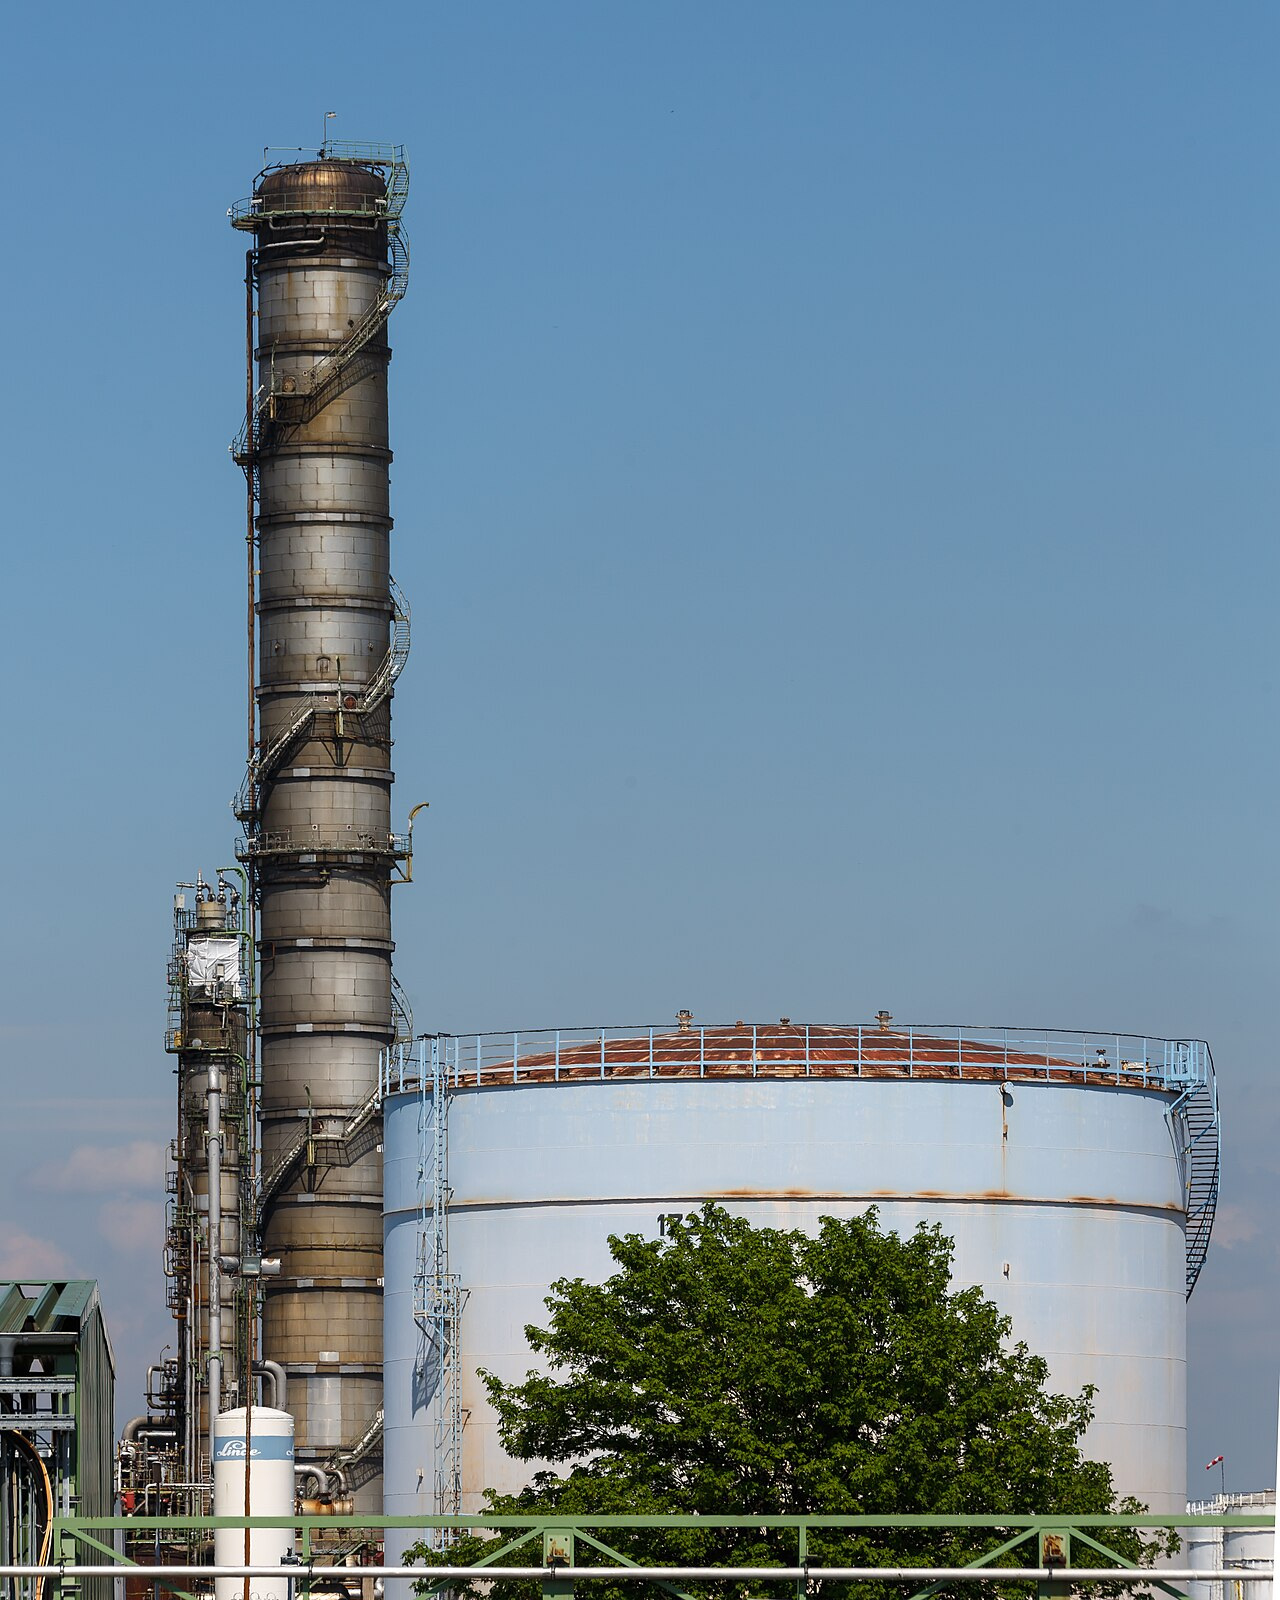
\includegraphics[width=\linewidth]{images/book3/refinery-column.jpg}
\end{minipage}

{\small बाएँ: एक प्लेट स्तंभ। द्रव हर प्लेट के आर-पार बहता है और
अधोवाहिनी से नीचे की प्लेट पर उतरता है; वाष्प प्लेटों से होकर ऊपर उठती है और
द्रव में से बुदबुदाती है। संघनित वाष्प का एक भाग पश्चवाह के रूप में लौटता है;
तली का पुनःक्वथित्र वाष्प प्रदान करता है। दाएँ: किसी रिफ़ाइनरी का
आसवन स्तंभ (कोलोन, 2014), जिसमें दर्जनों प्लेटें होती हैं। (छायाचित्र: सीईफ़ोटो,
ऊवे अरानास, CC BY-SA 3.0, विकिमीडिया कॉमन्स।)}
\end{omfigure}

\begin{proposition}[फ़ेंस्के समीकरण]\label{prop:b2:liquid-vapour-diagrams:fenske}
पूर्ण पश्चवाह पर, स्थिर आपेक्षिक वाष्पशीलता $\alpha$ के साथ,
तली के द्रव $x_B$ से आसुत $x_D$ तक जाने के लिए आवश्यक
\omterm{def:b2:liquid-vapour-diagrams:fractional-distillation}{सैद्धांतिक प्लेटों} की संख्या कम से कम यह है:
\[
  N_{\min} = \frac{1}{\ln\alpha}\,\ln\!\left[\frac{x_D}{1 - x_D}\cdot\frac{1 - x_B}{x_B}\right] .
\]
\end{proposition}

\begin{proof}
प्लेटों को तली से क्रमांकित कीजिए, पुनःक्वथित्र प्लेट 1 है। पूर्ण पश्चवाह पर
प्लेट $k + 1$ पर नीचे आने वाले द्रव का संघटन प्लेट $k$ से निकलने वाली
वाष्प जैसा है: $x_{k+1} = y_k$। $r = x/(1 - x)$ के साथ हर प्लेट
$r(y_k) = \alpha\,r(x_k)$ देती है, अतः $r(x_{k+1}) = \alpha\,r(x_k)$, और $N$
प्लेटों के बाद संघनित वाष्प के लिए $r(x_D) = \alpha^N r(x_B)$। लघुगणक लेने पर
$N$ मिलता है। परिमित पश्चवाह के साथ नीचे बहता द्रव ऊपर उठती वाष्प से
कम समृद्ध होता है, हर प्लेट कम समृद्ध करती है, और अधिक प्लेटें चाहिए।
\end{proof}

$(x, y)$ आरेख पर यही रचना साम्य वक्र और
विकर्ण $y = x$ के बीच एक सीढ़ी है: हर पायदान एक \omterm{def:b2:liquid-vapour-diagrams:fractional-distillation}{सैद्धांतिक
प्लेट} है।

\begin{omfigure}
\begin{tikzpicture}
\begin{axis}[width=0.55\linewidth, height=0.55\linewidth, xmin=0, xmax=1,
  ymin=0, ymax=1, axis x line=bottom, axis y line=left,
  xlabel={$x$ (बेन्ज़ीन, द्रव)}, ylabel={$y$ (बेन्ज़ीन, वाष्प)},
  tick label style={font=\small}, label style={font=\small}]
\addplot[omThm, thick] table[x=x, y=y] {figdata/out/bachelor-2-liquid-vapour-f-eq.dat};
\addplot[black!50] coordinates {(0,0) (1,1)};
\addplot[omDef, thick] table[x=x, y=y] {figdata/out/bachelor-2-liquid-vapour-f.dat};
\draw[densely dotted] (axis cs:0.95,0) -- (axis cs:0.95,0.95);
\draw[densely dotted] (axis cs:0.05,0) -- (axis cs:0.05,0.05);
\node[font=\scriptsize, anchor=south east] at (axis cs:0.945,0.02) {$x_D$};
\node[font=\scriptsize, anchor=south west] at (axis cs:0.05,0.02) {$x_B$};
\end{axis}
\end{tikzpicture}

{\small बेन्ज़ीन--टॉलूईन के लिए पूर्ण पश्चवाह पर प्लेटें, 0.95 के आसुत से
नीचे की ओर: हर क्षैतिज पायदान एक वाष्प से उसके साथ साम्य वाले द्रव तक जाता है
(एक प्लेट), हर ऊर्ध्वाधर पायदान उस द्रव से नीचे की प्लेट की
वाष्प तक। सात पायदान द्रव को $x_B = 0.05$ से नीचे ले जाते हैं;
फ़ेंस्के का सूत्र 6.5 देता है।}
% ledger: antoine:benzene.A, antoine:toluene.A (computed in figdata/bachelor-2/liquid-vapour.py)
\end{omfigure}

\begin{proposition}[स्तंभ स्थिरक्वाथी को पार नहीं कर सकता]\label{prop:b2:liquid-vapour-diagrams:azeotrope-limit}
\omterm{def:b2:liquid-vapour-diagrams:azeotrope}{स्थिरक्वाथी} वाले मिश्रण में, \omterm{def:b2:liquid-vapour-diagrams:azeotrope}{स्थिरक्वाथी} संघटन के एक ओर
पोषित स्तंभ अधिक से अधिक एक सिरे पर \omterm{def:b2:liquid-vapour-diagrams:azeotrope}{स्थिरक्वाथी} और दूसरे सिरे पर उस ओर का शुद्ध घटक
देता है।
\end{proposition}

\begin{proof}
\omterm{def:b2:liquid-vapour-diagrams:azeotrope}{स्थिरक्वाथी} पर साम्य वक्र विकर्ण से मिलता है: $y = x$। उसके निकट
सीढ़ी का हर पायदान लुप्तप्राय छोटा हो जाता है, इसलिए प्लेटों की कोई परिमित संख्या
उस तक नहीं पहुँचती, और कोई उसे पार नहीं करती।
\end{proof}

\begin{method}[प्रभाजी आसवन का पूर्वानुमान]\label{met:b2:liquid-vapour-diagrams:predict-distillation}
\begin{enumerate}
  \item \omterm{def:b2:liquid-vapour-diagrams:binary-diagram}{समदाबी आरेख} पर फ़ीड से पहुँच में न्यूनतम क्वथन बिंदु
        खोजिए: कोई शुद्ध घटक या \omterm{def:b2:liquid-vapour-diagrams:azeotrope}{धनात्मक स्थिरक्वाथी}। वह
        शीर्ष से निकलता है।
  \item उसी ओर का उच्चतम क्वथन बिंदु (शुद्ध घटक या
        \omterm{def:b2:liquid-vapour-diagrams:azeotrope}{ऋणात्मक स्थिरक्वाथी}) क्वथित्र में बचा रहता है।
  \item \omterm{def:b2:liquid-vapour-diagrams:azeotrope}{स्थिरक्वाथी} होने पर देखिए कि फ़ीड उसकी किस ओर है: केवल उसी
        ओर का शुद्ध घटक प्राप्त किया जा सकता है।
  \item प्लेटों की संख्या के लिए फ़ेंस्के सूत्र या सीढ़ी का उपयोग कीजिए,
        फिर वास्तव में प्रयुक्त परिमित पश्चवाह के लिए प्लेटें जोड़िए।
\end{enumerate}
\end{method}

0.881 से कम पर पोषित एथेनॉल और जल के लिए शीर्ष अधिक से अधिक
\omterm{def:b2:liquid-vapour-diagrams:azeotrope}{स्थिरक्वाथी} देता है और तली जल: कोई स्तंभ निरपेक्ष एथेनॉल नहीं देता। अंतिम
प्रतिशत को सुखाने के लिए दूसरी विधि चाहिए --- जल का अधिशोषण करने वाली आण्विक चलनी, या
\omterm{def:b2:liquid-vapour-diagrams:azeotrope}{स्थिरक्वाथी} को तोड़ने के लिए मिलाया गया एक तीसरा घटक।

\begin{omfigure}
\begin{tikzpicture}[font=\small, scale=0.95, >={Stealth}]
  \pic[transform shape] at (0,0) {heatingmantle};
  \pic[transform shape] at (0,0) {rbflask={0.45}{orange!25}};
  \foreach \x/\y in {-0.35/0.25,0.05/0.18,0.35/0.3}
    \fill[black!55] (\x,\y) circle (0.06);
  % Vigreux column from the flask neck (0,3) to (0,6)
  \draw[om glass] (-0.22,3.0) -- (-0.22,6.0) (0.22,3.0) -- (0.22,6.0);
  \foreach \yy in {3.4,3.9,4.4,4.9,5.4} {
    \draw[om glass] (-0.22,\yy) -- (-0.06,\yy+0.18) -- (-0.22,\yy+0.3);
    \draw[om glass] (0.22,\yy+0.15) -- (0.06,\yy+0.33) -- (0.22,\yy+0.45);
  }
  \pic[transform shape] (s) at (0,6.0) {stillhead};
  \pic[transform shape] at ($(s-top)+(0,-0.75)$) {thermometer};
  \pic[transform shape, rotate=-20] (c) at (s-arm) {liebig={3.4}};
  % ground-glass joint between the head's side arm and the condenser
  \draw[om glass, fill=white, rotate around={-20:(s-arm)}] ($(s-arm)+(-0.12,-0.17)$) rectangle ($(s-arm)+(0.14,0.17)$);
  \coordinate (cend) at ($(s-arm)+(-20:3.4)$);
  \pic[transform shape] (a) at (cend) {adapter};
  \pic[transform shape] at ($(a-tip)+(0,-2.4)$) {erlenmeyer={0.22}{orange!12}};
  \draw[<-, omProp, thick] (-0.25,4.6) -- (-1.6,4.6) node[left, text=black,
    align=right] {विग्रो स्तंभ\\ (खाँचे संपर्कों को\\ कई गुना करते हैं)};
  \draw[<-, omProp, thick] (0.12,6.72) -- (-1.4,7.4) node[left, text=black,
    align=right] {तापमापी का बल्ब\\ पार्श्व भुजा के स्तर पर};
  \draw[<-, omProp, thick] (1.08,0.3) -- (2.3,-0.2) node[right, text=black]
    {तापन आवरण};
  \draw[<-, omProp, thick] ($(a-tip)+(0.75,-2.0)$) -- ++(1.0,0.2)
    node[right, text=black] {आसुत};
\end{tikzpicture}

{\small प्रयोगशाला में \omterm{def:b2:liquid-vapour-diagrams:fractional-distillation}{प्रभाजी आसवन}। फ़्लास्क और शीर्ष के बीच का विग्रो स्तंभ
कुछ \omterm{def:b2:liquid-vapour-diagrams:fractional-distillation}{सैद्धांतिक प्लेटों} का काम करता है: वाष्प उसके खाँचों पर संघनित होती है
और ऊपर जाते हुए फिर वाष्पित होती है। शीर्ष पर ताप
सबसे वाष्पशील घटक के क्वथनांक पर तब तक बना रहता है जब तक वह आसवित होता है, फिर
बढ़ता है।}
\end{omfigure}

\begin{inthelab}[प्रभाजी आसवन द्वारा दो द्रवों का पृथक्करण]
फ़्लास्क अधिक से अधिक आधा भरा जाता है, क्वथन-पत्थरों के साथ, और धीरे-धीरे गर्म किया जाता है
ताकि संघनित होती वाष्प का वलय स्तंभ पर धीरे-धीरे चढ़े: तेज़ तापन से
भर गया स्तंभ अपनी प्लेटें खो देता है। शीर्ष का ताप हर
कुछ मिलीलीटर पर दर्ज किया जाता है; जब वह बढ़ने लगता है तो ग्राही बदल दिया जाता है (हर ताप-चरण
पर एक \textit{अंश} संग्रहित होता है), और फ़्लास्क के सूखने से पहले तापन
रोक दिया जाता है।
\end{inthelab}

\section{आंशिक रूप से मिश्रणीय और अमिश्रणीय द्रव}

\begin{definition}[मिश्रणीयता अंतराल]\label{def:b2:liquid-vapour-diagrams:miscibility-gap}
\emph{मिश्रणीयता अंतराल}\index{मिश्रणीयता अंतराल} समग्र
संघटनों का वह परिसर है जिसमें दो द्रव, दिए गए ताप पर, दो
द्रव परतों में अलग हो जाते हैं, जिनमें से हर एक दूसरे घटक से संतृप्त होती है।
\emph{विषम-स्थिरक्वाथी}\index{विषम-स्थिरक्वाथी} ऐसे
द्वि-परती द्रव का क्वथनांक है: दोनों द्रव परतें और वाष्प नियत
ताप पर और नियत वाष्प संघटन के साथ सह-अस्तित्व रखती हैं।
\end{definition}

\omterm{def:b2:liquid-vapour-diagrams:miscibility-gap}{विषम-स्थिरक्वाथी} पर दो घटक तीन प्रावस्थाओं में होते हैं: नियत
दाब पर \omterm{def:b2:equilibrium-shifts:variance}{स्वातंत्र्य कोटि} $2 + 2 - 3 - 1 = 0$ है। ताप
स्थिर रहता है, शुद्ध द्रव के क्वथनांक की तरह, जब तक दोनों परतें
बनी रहती हैं।

\begin{omfigure}
\begin{tikzpicture}[font=\small, x=6cm, y=0.08cm]
  \draw[->] (0,0) -- (1.05,0) node[right] {$x$};
  \draw[->] (0,0) -- (0,62) node[above] {$T$};
  \node[below] at (0,0) {2}; \node[below] at (1,0) {1};
  % boiling points: 2 at 50, 1 at 42; heteroazeotrope at 25 with layers 0.1 and 0.85, vapour 0.6
  \draw[omliquidus] (0,50) .. controls (0.04,38) and (0.08,30) .. (0.1,25);
  \draw[omliquidus] (1,42) .. controls (0.95,34) and (0.9,28) .. (0.85,25);
  \draw[omsolidus] (0,50) .. controls (0.25,46) and (0.5,35) .. (0.6,25);
  \draw[omsolidus] (1,42) .. controls (0.9,37) and (0.7,30) .. (0.6,25);
  \draw[thick] (0.1,25) -- (0.85,25);
  \draw[omliquidus] (0.1,25) -- (0.07,2);
  \draw[omliquidus] (0.85,25) -- (0.9,2);
  \fill (0.6,25) circle[radius=2pt];
  \node[font=\scriptsize] at (0.47,6) {दो द्रव परतें};
  \node[font=\scriptsize] at (0.5,55) {वाष्प};
  \node[font=\scriptsize] at (0.035,12) {L$_2$};
  \node[font=\scriptsize] at (0.96,12) {L$_1$};
  \node[font=\scriptsize, align=center] at (0.3,33) {L$_2$ + V};
  \node[font=\scriptsize, anchor=west] at (1.06,36) {L$_1$ + V};
  \draw[thin] (1.06,36) -- (0.86,29.5);
  \node[font=\scriptsize, anchor=north] at (0.6,24) {विषम-स्थिरक्वाथी};
\end{tikzpicture}

{\small दो आंशिक रूप से मिश्रणीय द्रवों का व्यवस्था-रूप \omterm{def:b2:liquid-vapour-diagrams:binary-diagram}{समदाबी आरेख}।
\omterm{def:b2:liquid-vapour-diagrams:miscibility-gap}{विषम-स्थिरक्वाथी} ताप से नीचे द्रव संघटनों के एक विस्तृत परिसर (\omterm{def:b2:liquid-vapour-diagrams:miscibility-gap}{मिश्रणीयता अंतराल}) में
दो परतों L$_1$ और L$_2$ में बँट जाता है; क्षैतिज
रेखा पर दोनों परतें साथ-साथ उबलकर नियत संघटन वाली वाष्प (बिंदु)
देती हैं।}
\end{omfigure}

\begin{definition}[भाप आसवन]\label{def:b2:liquid-vapour-diagrams:steam-distillation}
\emph{भाप आसवन}\index{भाप आसवन} जल के साथ अमिश्रणीय किसी
द्रव का उसमें भाप प्रवाहित करके किया गया आसवन है: मिश्रण दोनों द्रवों के
क्वथनांकों से नीचे उबलता है, और आसुत
दो परतों में अलग हो जाता है।
\end{definition}

\omterm{def:b2:liquid-vapour-diagrams:steam-distillation}{भाप आसवन} विद्यालय के खंड के जल-आसवन से केवल उस ढंग में भिन्न है
जिससे जल लाया जाता है: पदार्थ को जल में उबालने के बजाय पदार्थ में से
भाप प्रवाहित की जाती है। ऊष्मागतिकी वही है।

\begin{proposition}[दो अमिश्रणीय द्रवों का क्वथन]\label{prop:b2:liquid-vapour-diagrams:steam}
संपर्क में दो अमिश्रणीय द्रव उस ताप पर उबलते हैं जहाँ उनके
वाष्प दाबों का योग बाह्य दाब के बराबर हो, $p_1^*(T) + p_2^*(T) =
p$, जो दोनों क्वथनांकों से नीचे है। आसुत में दोनों द्रव
इस द्रव्यमान अनुपात में होते हैं:
\[
  \frac{m_1}{m_2} = \frac{p_1^*\,M_1}{p_2^*\,M_2} .
\]
\end{proposition}

\begin{proof}
हर शुद्ध द्रव दूसरे की मात्रा चाहे जो हो, अपना स्वयं का वाष्प दाब लगाता है:
दोनों परतों के ऊपर कुल दाब $p_1^* + p_2^*$ है, जो
उस ताप पर $p$ तक पहुँचता है जहाँ हर $p_i^*$, $p$ से छोटा है। वाष्प में
मात्राएँ आंशिक दाबों के समानुपाती होती हैं, $n_1/n_2 =
p_1^*/p_2^*$; $M_1/M_2$ से गुणा कीजिए।
\end{proof}

\begin{omfigure}
\begin{tikzpicture}
\begin{axis}[width=0.6\linewidth, height=5.5cm, xmin=70, xmax=100, ymin=0, ymax=1.6,
  axis x line=bottom, axis y line=left, xlabel={$T$ (\unit{\degreeCelsius})},
  ylabel={$p$ (\unit{bar})}, tick label style={font=\small},
  label style={font=\small}, clip=false]
\addplot[omProp, thick] table[x=t, y=ptol] {figdata/out/bachelor-2-liquid-vapour-e.dat};
\addplot[omDef, thick] table[x=t, y=pwat] {figdata/out/bachelor-2-liquid-vapour-e.dat};
\addplot[black, very thick] table[x=t, y=psum] {figdata/out/bachelor-2-liquid-vapour-e.dat};
\draw[densely dashed] (axis cs:70,1.013) -- (axis cs:100,1.013) node[right, font=\scriptsize] {\qty{1.013}{bar}};
\draw[densely dotted] (axis cs:84.3,0) -- (axis cs:84.3,1.013);
\node[font=\scriptsize, anchor=south east] at (axis cs:84.3,1.05) {\qty{84.3}{\degreeCelsius}};
\node[font=\scriptsize, anchor=west] at (axis cs:96,1.45) {योग};
\node[font=\scriptsize, omDef, anchor=south] at (axis cs:77,0.46) {जल};
\node[font=\scriptsize, omProp, anchor=north west] at (axis cs:88,0.5) {टॉलूईन};
\end{axis}
\end{tikzpicture}

{\small टॉलूईन और जल, अमिश्रणीय: हर द्रव के वाष्प दाब और
उनका योग। दोनों परतें \qty{84.3}{\degreeCelsius} पर साथ-साथ उबलती हैं, जो
जल (\qty{100}{\degreeCelsius}) और टॉलूईन (\qty{110.6}{\degreeCelsius}) से नीचे है;
आसुत प्रति ग्राम जल 4.1 g टॉलूईन ले जाता है।}
% ledger: antoine:toluene.A, antoine:water.A, aw:C, aw:H, aw:O (computed in figdata/bachelor-2/liquid-vapour.py)
\end{omfigure}

पादप सुगंधों के भारी, नाज़ुक अणु इसी प्रकार \qty{100}{\degreeCelsius} से
थोड़ा नीचे आसवित होते हैं, अपने स्वयं के क्वथनांकों से कहीं नीचे, बहुत कम
विघटन के साथ; क़ीमत है ऐसा आसुत जो अधिकांशतः जल होता है।

\section{अभ्यास}

\begin{exercise}[$\star$]\label{exo:b2:liquid-vapour-diagrams:1}
समदाबी बेन्ज़ीन--टॉलूईन आरेख पर शुद्ध द्रवों के क्वथनांक, संघटन 0.2 वाले
द्रव का \omterm{def:b2:liquid-vapour-diagrams:bubble-dew}{बुलबुला बिंदु} और उसकी पहली वाष्प का संघटन
पढ़िए।
\end{exercise}

\begin{exercise}[$\star$]\label{exo:b2:liquid-vapour-diagrams:2}
\qty{80}{\degreeCelsius} पर बेन्ज़ीन और टॉलूईन के वाष्प दाब
\qty{1.010}{bar} और \qty{0.388}{bar} हैं। सममोलर द्रव के लिए वह
दाब जिस पर वह उबलना आरंभ करता है, और वाष्प का संघटन परिकलित कीजिए।
\end{exercise}

\begin{exercise}[$\star$]\label{exo:b2:liquid-vapour-diagrams:3}
समग्र संघटन 0.30 वाले मिश्रण के \qty{10}{mol} ऐसे ताप पर हैं
जहाँ द्रव का संघटन 0.20 और वाष्प का 0.45 है। हर प्रावस्था की
मात्राएँ परिकलित कीजिए।
\end{exercise}

\begin{exercise}[$\star$]\label{exo:b2:liquid-vapour-diagrams:4}
नियत दाब पर बेन्ज़ीन--टॉलूईन मिश्रण की \omterm{def:b2:equilibrium-shifts:variance}{स्वातंत्र्य कोटि} परिकलित कीजिए: (a) पूरा द्रव; (b)
उबलता हुआ; (c) किसी \omterm{def:b2:liquid-vapour-diagrams:azeotrope}{स्थिरक्वाथी} पर, ऐसे युग्म के लिए जिसमें वह हो।
\end{exercise}

\begin{exercise}[$\star\star$]\label{exo:b2:liquid-vapour-diagrams:5}
\qty{1.013}{bar} पर संघटन 0.30 वाली बेन्ज़ीन--टॉलूईन वाष्प का \omterm{def:b2:liquid-vapour-diagrams:bubble-dew}{ओसांक} प्रयास द्वारा ज्ञात
कीजिए, $p^*_{\text{बेन्ज़ीन}}$ और $p^*_{\text{टॉलूईन}}$
(\unit{bar}) के साथ: \qty{100}{\degreeCelsius} पर 1.80 और 0.742,
\qty{105}{\degreeCelsius} पर 2.057 और 0.861। पहली बूँद का संघटन दीजिए।
\end{exercise}

\begin{exercise}[$\star\star$]\label{exo:b2:liquid-vapour-diagrams:6}
एक सममोलर बेन्ज़ीन--टॉलूईन मिश्रण का सरल आसवन (बिना स्तंभ) किया जाता है। आसुत की
पहली बूँदों का संघटन क्या है? आसवन आगे बढ़ने पर आसुत का ताप और
संघटन कैसे बदलते हैं? पृथक्करण
कमज़ोर क्यों है?
\end{exercise}

\begin{exercise}[$\star\star$]\label{exo:b2:liquid-vapour-diagrams:7}
एथेनॉल में 0.05 मोल अंश वाली एक वाइन का बहुत दक्ष स्तंभ के साथ \omterm{def:b2:liquid-vapour-diagrams:fractional-distillation}{प्रभाजी आसवन}
किया जाता है। शीर्ष से क्या निकलता है, और क्वथित्र में क्या बचता है?
0.95 मोल अंश वाले मिश्रण के लिए यही प्रश्न।
\end{exercise}

\begin{exercise}[$\star\star$]\label{exo:b2:liquid-vapour-diagrams:8}
किसी पादप सुगंध का एक घटक (मोलर द्रव्यमान \qty{136}{g/mol}) लगभग
\qty{97}{\degreeCelsius} पर \qty{0.10}{bar} का वाष्प दाब रखता है, जहाँ जल का वाष्प दाब
\qty{0.91}{bar} है (अभ्यास के आँकड़े)। \qty{1.013}{bar} के अंतर्गत \omterm{def:b2:liquid-vapour-diagrams:steam-distillation}{भाप
आसवन} किस ताप पर चलता है, और प्रति ग्राम जल सुगंध के कितने ग्राम
संग्रहित होते हैं?
\end{exercise}

\begin{exercise}[$\star\star$]\label{exo:b2:liquid-vapour-diagrams:9}
आंशिक रूप से मिश्रणीय द्रवों के व्यवस्था-रूप आरेख पर वर्णन कीजिए कि
समग्र संघटन 0.4 वाले द्वि-परती मिश्रण को कमरे के ताप से तब तक गर्म करने पर
जब तक वह पूरा वाष्प न हो जाए, क्या होता है: प्रावस्थाएँ, ताप, और पहली
वाष्प का संघटन।
\end{exercise}

\begin{exercise}[$\star\star\star$]\label{exo:b2:liquid-vapour-diagrams:10}
$\alpha = 2.47$ के साथ 0.99 के आसुत और 0.01 की तली के लिए \omterm{def:b2:liquid-vapour-diagrams:fractional-distillation}{सैद्धांतिक प्लेटों} की
न्यूनतम संख्या परिकलित कीजिए। 0.95 और 0.05 के लिए आवश्यक 6.5 से तुलना
कीजिए, और शुद्धता की क़ीमत पर टिप्पणी कीजिए।
\end{exercise}

\begin{exercise}[$\star\star\star$]\label{exo:b2:liquid-vapour-diagrams:11}
बेन्ज़ीन--टॉलूईन के \omterm{def:b2:liquid-vapour-diagrams:binary-diagram}{समदाबी आरेख} और एंटोइन समीकरणों से समझाइए कि
\qty{80}{\degreeCelsius} पर \omterm{def:b2:liquid-vapour-diagrams:binary-diagram}{समतापी आरेख} कैसे प्राप्त होता है,
और उस पर द्रव क्षेत्र ऊपर क्यों है।
\end{exercise}

\begin{exercise}[$\star\star\star$]\label{exo:b2:liquid-vapour-diagrams:12}
संबंध $d\ln p = (y - x)\,dy/[y(1 - y)]$ से आरंभ करके दिखाइए कि नियत
ताप पर कुल दाब $x$ के साथ वहाँ बढ़ता है जहाँ वाष्प
घटक 1 में द्रव से अधिक समृद्ध है, और निष्कर्ष निकालिए कि \omterm{def:b2:chemical-potential:ideal-mixture}{आदर्श मिश्रण} में कोई
\omterm{def:b2:liquid-vapour-diagrams:azeotrope}{स्थिरक्वाथी} नहीं होता।
\end{exercise}

\section{समस्या: बेन्ज़ीन और टॉलूईन के लिए एक स्तंभ}

\begin{problem}[{सप्ताहांत समस्या --- एंटोइन समीकरणों से बेन्ज़ीन और
टॉलूईन का समदाबी आरेख, एक फ़्लैश और उत्तोलक नियम, पूर्ण पश्चवाह पर स्तंभ
की प्लेटों की न्यूनतम संख्या, और वह सीमा जो स्थिरक्वाथी
लगाता है}]
\label{pb:b2:liquid-vapour-diagrams:1}
आँकड़े: एंटोइन समीकरण, $\log_{10}(p^*/\unit{bar}) = A - B/(T + C)$, जहाँ $T$
केल्विन में है: बेन्ज़ीन $A = 4.01814$, $B = \qty{1203.835}{K}$, $C =
\qty{-53.226}{K}$; टॉलूईन $A = 4.07827$, $B = \qty{1343.943}{K}$, $C =
\qty{-53.773}{K}$। दाब \qty{1.013}{bar}; बेन्ज़ीन और टॉलूईन \omterm{def:b2:chemical-potential:ideal-mixture}{आदर्श
मिश्रण} बनाते हैं। एथेनॉल--जल \omterm{def:b2:liquid-vapour-diagrams:azeotrope}{स्थिरक्वाथी} में द्रव्यमान के अनुसार 95~\% एथेनॉल है।
% ledger: antoine:benzene.A, antoine:benzene.B, antoine:benzene.C, antoine:toluene.A, antoine:toluene.B, antoine:toluene.C, azeo:ethanol-water.w

\medskip
\noindent\textbf{भाग I --- आरेख।}
\begin{enumerate}
  \item \qty{1.013}{bar} पर बेन्ज़ीन और टॉलूईन के क्वथनांक परिकलित कीजिए।
  \item \qty{90}{\degreeCelsius} पर $p_1^*$ और $p_2^*$ परिकलित कीजिए।
  \item \qty{90}{\degreeCelsius} पर साम्य में द्रव और वाष्प के
        संघटन निकालिए।
  \item \qty{100}{\degreeCelsius} पर यही ($p_1^* = \qty{1.800}{bar}$, $p_2^* =
        \qty{0.742}{bar}$)।
  \item इन चार बिंदुओं और शुद्ध द्रवों से \omterm{def:b2:liquid-vapour-diagrams:binary-diagram}{समदाबी आरेख} का रेखाचित्र बनाइए।
  \item \qty{90}{\degreeCelsius} और
        \qty{95}{\degreeCelsius} के बीच प्रयास द्वारा सममोलर द्रव का \omterm{def:b2:liquid-vapour-diagrams:bubble-dew}{बुलबुला बिंदु},
        \qty{0.5}{\degreeCelsius} तक, ज्ञात कीजिए।
  \item उबलते मिश्रण की \omterm{def:b2:equilibrium-shifts:variance}{स्वातंत्र्य कोटि} परिकलित कीजिए और बताइए कि
        आरेख के लिए इसका क्या अर्थ है।
\end{enumerate}

\medskip
\noindent\textbf{भाग II --- एक फ़्लैश।}
\begin{enumerate}[resume]
  \item एक सममोलर फ़ीड को \qty{95}{\degreeCelsius} तक गर्म किया जाता है ($p_1^* =
        \qty{1.569}{bar}$, $p_2^* = \qty{0.636}{bar}$)। $x$ और $y$ परिकलित कीजिए।
  \item फ़ीड के \qty{100}{mol} के लिए द्रव और वाष्प की मात्राएँ परिकलित कीजिए।
  \item हर प्रावस्था में बेन्ज़ीन की मात्रा परिकलित कीजिए और संतुलन जाँचिए।
  \item बेन्ज़ीन का कितना अंश वाष्प में पुनःप्राप्त होता है?
  \item यदि फ़्लैश \qty{100}{\degreeCelsius} पर चलाया जाए तो क्या होता है?
  \item किस ताप पर फ़ीड पूरी तरह वाष्पित हो जाता है?
\end{enumerate}

\medskip
\noindent\textbf{भाग III --- स्तंभ।}
\begin{enumerate}[resume]
  \item आपेक्षिक वाष्पशीलता $\alpha$ परिभाषित कीजिए और बेन्ज़ीन के क्वथनांक
        पर इसे परिकलित कीजिए।
  \item टॉलूईन के क्वथनांक पर इसे परिकलित कीजिए।
  \item पूरे स्तंभ के लिए मान के रूप में ज्यामितीय माध्य लीजिए।
  \item दिखाइए कि \omterm{def:b2:liquid-vapour-diagrams:fractional-distillation}{सैद्धांतिक प्लेट} पर $y/(1 - y) = \alpha\,x/(1 - x)$।
  \item समझाइए कि पूर्ण पश्चवाह पर किसी प्लेट में प्रवेश करने वाले द्रव का
        संघटन नीचे की प्लेट से निकलने वाली वाष्प जैसा क्यों होता है।
  \item फ़ेंस्के का सूत्र व्युत्पन्न कीजिए।
  \item 0.95 के आसुत और 0.05 की तली के लिए \omterm{def:b2:liquid-vapour-diagrams:fractional-distillation}{सैद्धांतिक प्लेटों} की न्यूनतम संख्या
        परिकलित कीजिए।
  \item वास्तविक स्तंभ को इससे अधिक प्लेटें क्यों दी जाती हैं?
  \item अध्याय की सीढ़ी पर पायदान गिनिए और तुलना कीजिए।
\end{enumerate}

\medskip
\noindent\textbf{भाग IV --- एक \omterm{def:b2:liquid-vapour-diagrams:azeotrope}{स्थिरक्वाथी}।}
\begin{enumerate}[resume]
  \item एथेनॉल--जल \omterm{def:b2:liquid-vapour-diagrams:azeotrope}{स्थिरक्वाथी} में एथेनॉल का मोल अंश परिकलित कीजिए।
  \item 0.10 एथेनॉल वाला फ़ीड पचास प्लेटों वाले स्तंभ में प्रवेश करता है। शीर्ष और
        तली से क्या निकलता है?
  \item बेन्ज़ीन और टॉलूईन को 95~\% के उत्पादों में अलग करने के लिए आवश्यक
        \omterm{def:b2:liquid-vapour-diagrams:fractional-distillation}{सैद्धांतिक प्लेटों} की न्यूनतम संख्या बताइए।
\end{enumerate}
\end{problem}
